\documentclass[tikz,border=20pt]{standalone}
\usepackage[utf8]{inputenc}
\usepackage{tikz}
\usetikzlibrary{positioning, calc, arrows.meta, decorations.pathreplacing, shapes.multipart, patterns, fit, backgrounds, shadows}

% --- 配色方案 (Light Theme) ---
\definecolor{fixedblue}{RGB}{227, 242, 253}
\definecolor{offsetorange}{RGB}{255, 243, 224}
\definecolor{heapgreen}{RGB}{232, 245, 233}
\definecolor{garbagegrey}{RGB}{245, 245, 245}
\definecolor{linegrey}{RGB}{180, 180, 180}
\definecolor{alertred}{RGB}{211, 47, 47}
\definecolor{invariantblue}{RGB}{25, 118, 210}

% 代码块配色 (Go Style)
\definecolor{paperbg}{RGB}{255, 255, 255}
\definecolor{paperborder}{RGB}{220, 220, 220}
\definecolor{codetext}{RGB}{33, 33, 33}
\definecolor{codetype}{RGB}{0, 122, 204}
\definecolor{codekw}{RGB}{215, 58, 73}
\definecolor{commentgrey}{RGB}{106, 153, 85} % VSCode green comment

\begin{document}

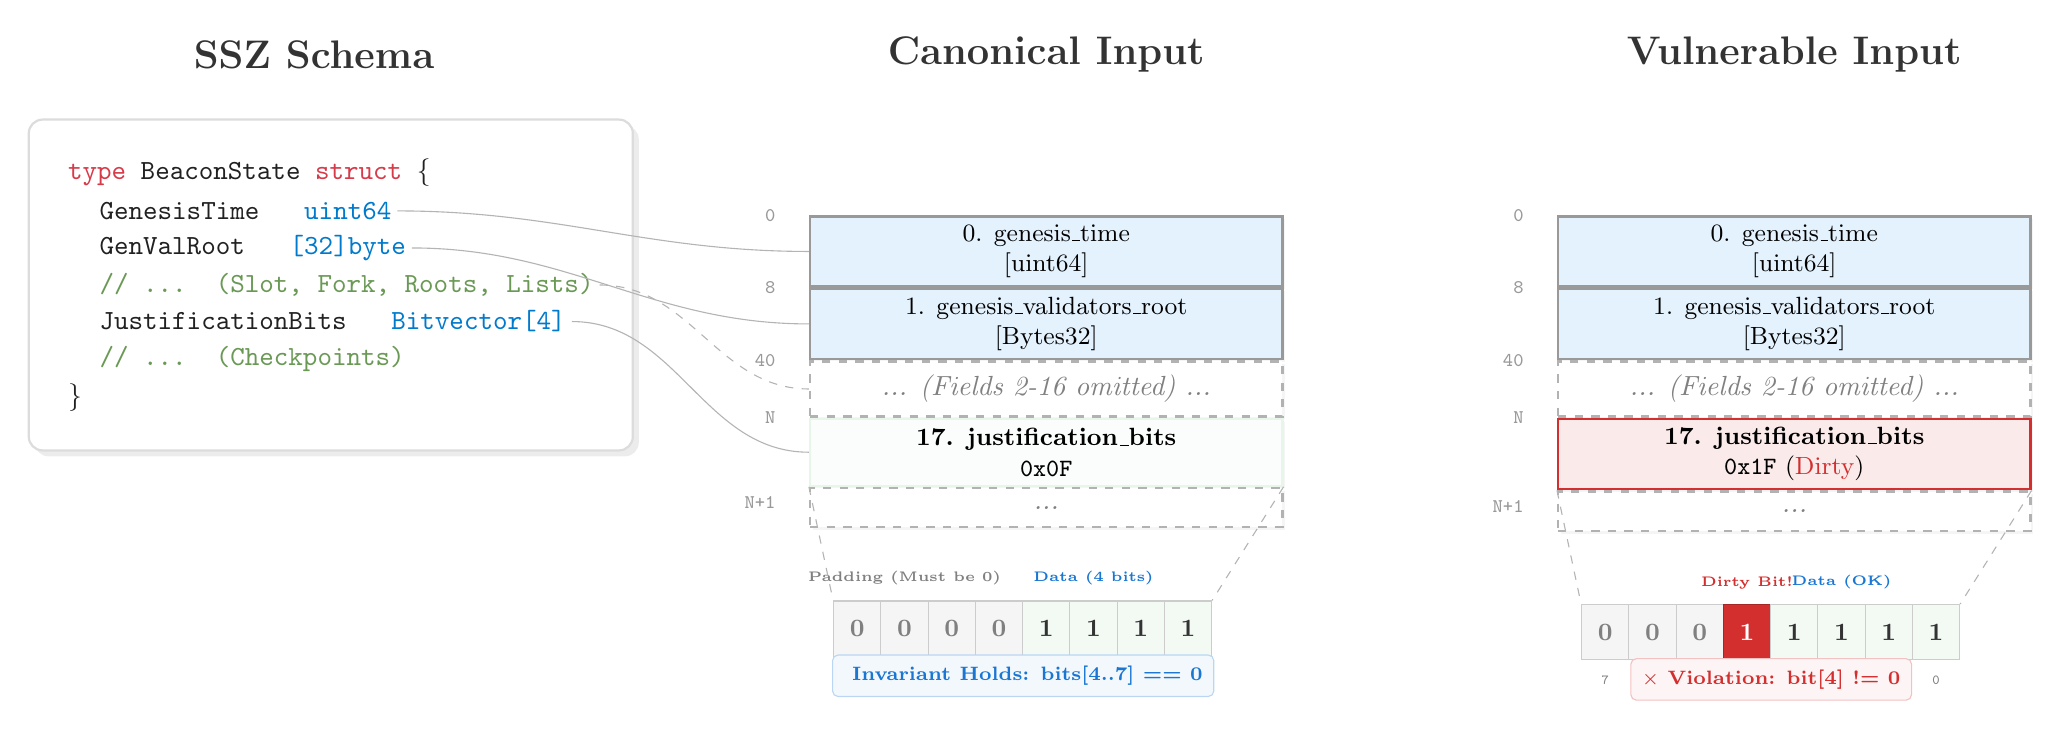
\begin{tikzpicture}[
    font=\sffamily,
    % --- 样式定义 ---
    byteblock/.style={
        rectangle,
        draw=black!40,
        thick,
        minimum width=6.0cm,
        align=center,
        inner sep=3pt,
        drop shadow={opacity=0.08, shadow xshift=1pt, shadow yshift=-1pt}
    },
    fixed/.style={byteblock, fill=fixedblue, minimum height=0.85cm, font=\small},
    offset/.style={byteblock, fill=offsetorange, minimum height=1.1cm, font=\bfseries\small},
    heap/.style={byteblock, fill=heapgreen, minimum height=1.4cm},
    % 新增：省略块样式
    skipped/.style={
        byteblock, 
        fill=white, 
        draw=black!30, 
        dashed, 
        minimum height=0.7cm, 
        font=\itshape\color{gray}
    },
    index/.style={
        font=\scriptsize\ttfamily,
        color=gray!80,
        anchor=east,
        xshift=-0.3cm
    },
    typefont/.style={
        font=\tiny\itshape,
        color=black!50
    },
    % 代码行样式
    codeline/.style={
        font=\bfseries\ttfamily, 
        text=codetext,
        anchor=west,
        align=left,
        inner sep=2pt,
        minimum height=0.45cm
    },
    invariant/.style={
        rectangle,
        draw=invariantblue!30,
        fill=invariantblue!5,
        text=invariantblue,
        font=\scriptsize\bfseries,
        align=left,
        rounded corners=2pt,
        inner sep=4pt,
        anchor=west
    },
    % Bit 样式
    bitbox/.style={
        rectangle,
        draw=black!20,
        minimum width=0.6cm,
        minimum height=0.7cm,
        align=center,
        font=\small\bfseries,
        inner sep=0pt,
        fill=white
    }
]

% =========================================
% 1. MIDDLE: CANONICAL LAYOUT
% =========================================
\begin{scope}[local bounding box=leftscope]
    \node[font=\Large\bfseries, color=black!80] at (0, 2.5) {Canonical Input};

    % --- FIXED PART ---
    \node[fixed] (l_f0) {0. genesis\_time \\ \typefont{[uint64]}}; 
    \node[index] at (l_f0.north west) {0};

    \node[fixed, below=0pt of l_f0] (l_f1) {1. genesis\_validators\_root \\ \typefont{[Bytes32]}};
    \node[index] at (l_f1.north west) {8};

    % --- OMITTED FIELDS (Slot, Fork, Roots, etc.) ---
    \node[skipped, below=0pt of l_f1] (l_skip) {... (Fields 2-16 omitted) ...};
    \node[index] at (l_skip.north west) {40};

    % Target Field (Updated index to 17 based on BeaconState definition)
    \node[fixed, below=0pt of l_skip, fill=heapgreen!20, draw=heapgreen] (l_f2) {\textbf{17. justification\_bits} \\ \texttt{0x0F}};
    \node[index] at (l_f2.north west) {N};
    \node[index, anchor=north east] at (l_f2.south west) {\textbf{N+1}};
    
    % --- OMITTED FIELDS (Checkpoints) ---
    \node[skipped, below=0pt of l_f2, minimum height=0.5cm] (l_skip2) {...};

    % --- BIT ZOOM VIEW ---
    \begin{scope}[shift={($(l_f2.south) + (0, -1.8)$)}]
        \coordinate (bitstart) at (-2.4, 0);

        % Padding Bits
        \foreach \x/\val in {0/0, 1/0, 2/0, 3/0} {
            \node[bitbox, fill=garbagegrey, text=gray] (b\x) at ($(bitstart) + (\x*0.6, 0)$) {\val};
        }
        % Data Bits
        \foreach \x/\val in {4/1, 5/1, 6/1, 7/1} {
            \node[bitbox, fill=heapgreen!50, text=black!80] (b\x) at ($(bitstart) + (\x*0.6, 0)$) {\val};
        }

        % Labels
        \node[font=\tiny\bfseries, color=gray, above=2pt of b1] {Padding (Must be 0)};
        \node[font=\tiny\bfseries, color=invariantblue, above=2pt of b5] {Data (4 bits)};
        % Indices
        \node[font=\tiny\ttfamily, color=gray, below=2pt of b0] {7};
        \node[font=\tiny\ttfamily, color=gray, below=2pt of b7] {0};
        % Check
        \node[invariant, below=0.6cm of b3.east, anchor=center] (check_ok) {$\checkmark$ Invariant Holds: bits[4..7] == 0};
    \end{scope}

    \draw[dashed, linegrey] (l_f2.south west) -- (b0.north west);
    \draw[dashed, linegrey] (l_f2.south east) -- (b7.north east);
\end{scope}

% =========================================
% 0. LEFTMOST: GO STRUCT DEFINITION
% =========================================
\begin{scope}[xshift=-12.5cm]
    \node[font=\Large\bfseries, color=black!80] at (3.2, 2.5) {SSZ Schema};

    % 1. Struct Header
    \node[codeline] (struct_head) at (0, 1.0) {\textcolor{codekw}{type} BeaconState \textcolor{codekw}{struct} \{};

    % 2. Struct Fields
    \node[codeline, below=0pt of struct_head.south west, anchor=north west] (c_l_f0) {\hspace{0.4cm}GenesisTime \hspace{0.2cm} \textcolor{codetype}{uint64}};
    \node[codeline, below=0pt of c_l_f0.south west, anchor=north west] (c_l_f1) {\hspace{0.4cm}GenValRoot \hspace{0.2cm} \textcolor{codetype}{[32]byte}};
    
    % Insert Ellipsis for Go code
    \node[codeline, below=0pt of c_l_f1.south west, anchor=north west] (c_skip_code) {\hspace{0.4cm}\textcolor{commentgrey}{// ... (Slot, Fork, Roots, Lists)}};

    \node[codeline, below=0pt of c_skip_code.south west, anchor=north west] (c_l_f2) {\hspace{0.4cm}JustificationBits \hspace{0.2cm} \textcolor{codetype}{Bitvector[4]}};
    
    % Insert trailing ellipsis
    \node[codeline, below=0pt of c_l_f2.south west, anchor=north west] (c_skip_code2) {\hspace{0.4cm}\textcolor{commentgrey}{// ... (Checkpoints)}};

    % 3. Closing Brace
    \node[codeline, below=0pt of c_skip_code2.south west, anchor=north west] (struct_end) {\}};

    % 4. Background Window
    \begin{scope}[on background layer]
        \node[
            rectangle,
            draw=paperborder,
            thick,
            fill=paperbg,
            rounded corners=5pt,
            fit=(struct_head) (struct_end) (c_l_f0) (c_l_f1) (c_l_f2) (c_skip_code), 
            inner sep=12pt,
            drop shadow={opacity=0.15}
        ] (code_window) {};
    \end{scope}

    % 5. Connecting Lines
    \draw[linegrey, thin] (c_l_f0.east) edge[out=0, in=180] (l_f0.west);
    \draw[linegrey, thin] (c_l_f1.east) edge[out=0, in=180] (l_f1.west);
    \draw[linegrey, thin, dashed] (c_skip_code.east) edge[out=0, in=180] (l_skip.west);
    \draw[linegrey, thin] (c_l_f2.east) edge[out=0, in=180] (l_f2.west);
\end{scope}

% =========================================
% 2. RIGHT SIDE: VULNERABLE LAYOUT
% =========================================
\begin{scope}[xshift=9.5cm, local bounding box=rightscope]
    \node[font=\Large\bfseries, color=black!80] at (0, 2.5) {Vulnerable Input};

    % --- FIXED PART ---
    \node[fixed] (r_f0) {0. genesis\_time \\ \typefont{[uint64]}}; 
    \node[index] at (r_f0.north west) {0};

    \node[fixed, below=0pt of r_f0] (r_f1) {1. genesis\_validators\_root \\ \typefont{[Bytes32]}};
    \node[index] at (r_f1.north west) {8};

    % --- OMITTED FIELDS ---
    \node[skipped, below=0pt of r_f1] (r_skip) {... (Fields 2-16 omitted) ...};
    \node[index] at (r_skip.north west) {40};

    % Target Field (Dirty)
    \node[fixed, below=0pt of r_skip, fill=alertred!10, draw=alertred] (r_f2) {\textbf{17. justification\_bits} \\ \texttt{0x1F} (\textcolor{alertred}{Dirty})};
    \node[index] at (r_f2.north west) {N};
    \node[index, anchor=north east] at (r_f2.south west) {\textbf{N+1}};

    % --- OMITTED FIELDS ---
    \node[skipped, below=0pt of r_f2, minimum height=0.5cm] (r_skip2) {...};

    % --- BIT ZOOM VIEW ---
    \begin{scope}[shift={($(r_f2.south) + (0, -1.8)$)}]
        \coordinate (rbitstart) at (-2.4, 0);

        % Padding Bits
        \node[bitbox, fill=garbagegrey, text=gray] (rb0) at ($(rbitstart) + (0*0.6, 0)$) {0};
        \node[bitbox, fill=garbagegrey, text=gray] (rb1) at ($(rbitstart) + (1*0.6, 0)$) {0};
        \node[bitbox, fill=garbagegrey, text=gray] (rb2) at ($(rbitstart) + (2*0.6, 0)$) {0};
        % THE BAD BIT
        \node[bitbox, fill=alertred, text=white, draw=alertred!80!black] (rb3) at ($(rbitstart) + (3*0.6, 0)$) {1};
        % Data Bits
        \foreach \x/\val in {4/1, 5/1, 6/1, 7/1} {
            \node[bitbox, fill=heapgreen!50, text=black!80] (rb\x) at ($(rbitstart) + (\x*0.6, 0)$) {\val};
        }

        % Labels
        \node[font=\tiny\bfseries, color=alertred, above=2pt of rb3] {Dirty Bit!};
        \node[font=\tiny\bfseries, color=invariantblue, above=2pt of rb5] {Data (OK)};
        % Indices
        \node[font=\tiny\ttfamily, color=gray, below=2pt of rb0] {7};
        \node[font=\tiny\ttfamily, color=gray, below=2pt of rb7] {0};
        % Check
        \node[invariant, draw=alertred!30, fill=alertred!5, text=alertred, below=0.6cm of rb3.east, anchor=center] (check_fail) {$\times$ Violation: bit[4] != 0};
    \end{scope}

    \draw[dashed, linegrey] (r_f2.south west) -- (rb0.north west);
    \draw[dashed, linegrey] (r_f2.south east) -- (rb7.north east);
\end{scope}

\end{tikzpicture}
\end{document}